\section{Rappresentazione stato-spazio di sistemi dinamici}
\subsection{Descrizione matematica}
La descrizione generale che possiamo sempre dare per un sistema dinamico è la
seguente:
\begin{equation}
    \begin{cases}
        \dot{x}(t) = f(x(t), u(t)) \rightarrow \text{state equation} \\
        y(t) = g(x(t), u(t)) \rightarrow \text{output equation}
    \end{cases}
\end{equation}
Se le funzioni $f$ e $g$ dipende dalla variabile tempo, allora il sistema è detto \textbf{time-varying}, altrimenti è detto \textbf{time-invariant}.
Se $g$ non dipende esplicitamente da $u(t)$, allora il sistema è detto \textbf{strictly proper}.
Quando considero un sistema dinamico posso avere $n$ variabili di stato, $p$ ingressi e $q$ uscite.
Riassumendo, un sistema dinamico è descritto da:
\begin{equation}
    \begin{cases}
        \dot{x}(t) = f(x(t), u(t)) \\
        y(t) = g(x(t), u(t))
    \end{cases}
    \quad
    \begin{cases}
        x(t) \in \mathbb{R}^n \\
        u(t) \in \mathbb{R}^m \\
        y(t) \in \mathbb{R}^q
    \end{cases}
\end{equation}
Noi ci occuperemo di sistemi finiti-dimensionali, ovvero sistemi che hanno un numero finito di variabili di stato.
\begin{tcolorbox}[colback=yellow!10, colframe=black]
    \textbf{Esempio:}
    \newline
    \newline
    \begin{minipage}
        {0.5\textwidth}
        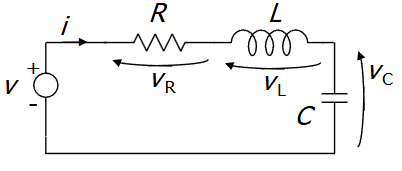
\includegraphics[width=0.9\linewidth]{foto/cph2/1.png}
    \end{minipage}
    \begin{minipage}
        {0.5\textwidth}
        Vogliamo descrivere il sistema dinamico rappresentato in figura.
        Partiamo da come si descrive il sistema dinamico in forma di sistema dinamico:
        \begin{equation}
            \begin{cases}
                \dot{x}(t) = f(x(t), u(t)) \\
                y(t) = g(x(t), u(t))
            \end{cases}
        \end{equation}

    \end{minipage}
    \newline
    Definisco ora le variabili di stato, ingresso e uscita:
    \[
        \begin{cases}
            x (t) =V (t)            \\
            u (t) = V_C (t)+V_R (t) \\
        \end{cases}
    \]
    Per ognuno degli oggetti del circuito, scrivo la legge di Kirchhoff:
    \[
        \begin{cases}
            V_R (t) = R i (t)                   \\
            V_L (t) = L \frac{di(t)}{dt}        \\
            V_C (t) = \frac{1}{C} \int i (t) dt \\
            i (t) = C \frac{dV_C (t)}{dt}
        \end{cases}
    \]
    Le nostre variabili di stato saranno quindi $x_1 (t) = V (t)$ e $x_2 (t) = i
        (t)$. Sostituisco ora le mie nella mia descrizione generale del sistema
    dinamico:
    \[
        \begin{cases}
            \dot{x}_1 (t) = \dot{V} (t) = \frac{1}{C} i (t) = \frac{1}{C} x_2 (t) \\
            \dot{x}_2 (t) = \dot{i} (t) = \frac{1}{L} u (t) - \frac{R}{L} i (t) - \frac{1}{L} V (t) = \frac{1}{L} u (t) - \frac{R}{L} x_2 (t) - \frac{1}{L} x_1 (t)
        \end{cases}
    \]
    Per quanto riguarda l'uscita, abbiamo che:
    \[
        y (t) = V_C (t) + V_R (t) = x_1 (t) + R x_2 (t)
    \]
\end{tcolorbox}